\section{Idea Progettuale}

\subsection{Ispirazione}

Visitando frequentemente questo luogo, che affascina per la presenza del lago, ho notato la scarsità di bar o zone ristoro, pur essendoci spazi verdi attrezzati per pic-nic. 
Ho quindi immaginato di potere riconvertire il rimessaggio barche in un bar chiosco.
Vista la sua collocazione ho pensato che il bar potesse offrire, oltre al servizio standard, anche un servizio take-away e cestini merenda da potersi consumare in riva al lago.

\begin{figure}[H]
	\centering
	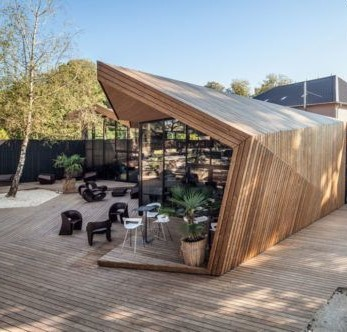
\includegraphics[width=0.8\textwidth]{image14}
	\caption{aaa}
	\label{fig:mesh1}
\end{figure}

Volevo realizzare una struttura  originale , che non fosse troppo statica e che non  stridesse con l’ambiente circostante .
Non volevo un posto totalmente  chiuso .
Ho quindi individuato un progetto che,  con  le sue due  pareti libere,  permette di avere sempre la visione del lago e la sensazione di essere in uno spazio aperto. 

\subsection{Struttura}

La struttura è larga 4,30 metri e lunga 5,40 metri  e costruita con legno di larice per il rivestimento , travi  IPE acciaio e chiusure trasparenti.

\begin{figure}[H]
	\centering
	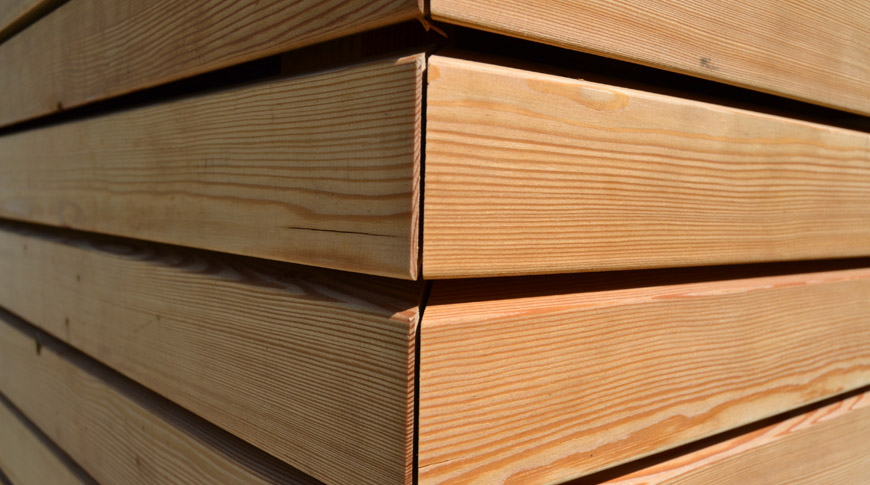
\includegraphics[width=0.8\textwidth]{image21}
	\caption{aaa}
	\label{fig:mesh1}
\end{figure}


Come rivestimento esterno di tutta la struttura ho scelto il larice perchè è un legno adatto ai rivestimenti. 

\begin{figure}[H]
	\centering
	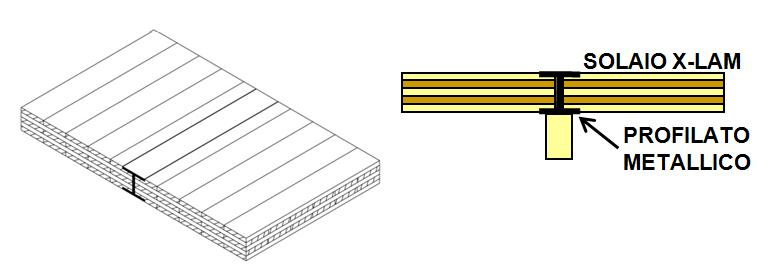
\includegraphics[width=0.8\textwidth]{image35}
	\caption{aaa}
	\label{fig:mesh1}
\end{figure}

l legno di larice è un ottimo legno per rivestimenti per esterni, grazie alle sue notevoli proprietà isolanti. Il legno di larice tende ad assumere una tonalità grigiastra con il passare del tempo e tale escursione cromatica che lo  rende particolarmente apprezzato . 
Inoltre ha una notevole durezza, resistenza alle sollecitazioni e un buon coefficiente di impermeabilità. 




Il lato nord è costituito da una parete di legno con due diverse inclinazioni, anche il lato ovest ,che si rivolge alla strada, è costituito da una parete di legno, mentre i lati est e sud sono aperti.
Tutta la struttura poggia su una pedana di legno.
I due lati aperti permettono il diretto accesso al bancone del bar e rendono la struttura integrata con l’ambiente che la circonda. 

La struttura è pensata per un uso estivo, visto che non offre tavoli al coperto. 
Ho previsto una chiusura dei lati aperti tramite una serranda orizzontale, 
in modo da chiudere il chiosco durante la notte o durante il periodo di non utilizzo. 

La parte frontale della struttura si sviluppa a partire dalla forma di un pentagono, mentre la parte posteriore relativa ad un guscio di protezione.

\begin{figure}[H]
	\centering
	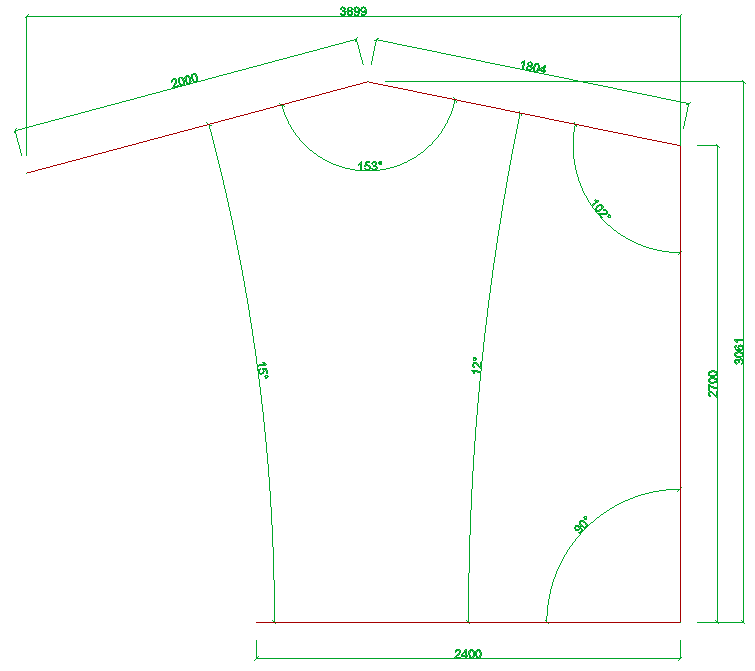
\includegraphics[width=0.8\textwidth]{image1}
	\caption{Vista laterale}
	\label{fig:mesh1}
\end{figure}

\begin{figure}[H]
	\centering
	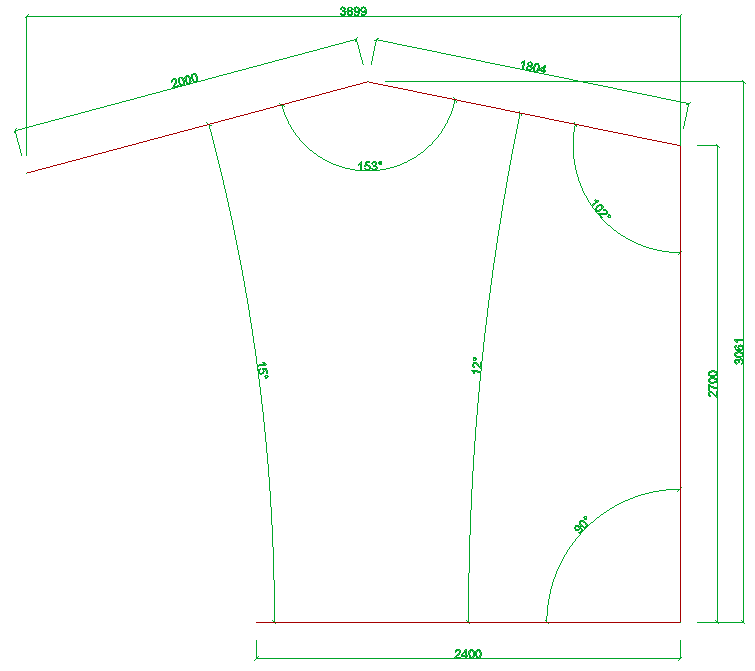
\includegraphics[width=0.8\textwidth]{image1}
	\caption{Vista posteriore}
	\label{fig:mesh1}
\end{figure}

\begin{figure}[H]
	\centering
	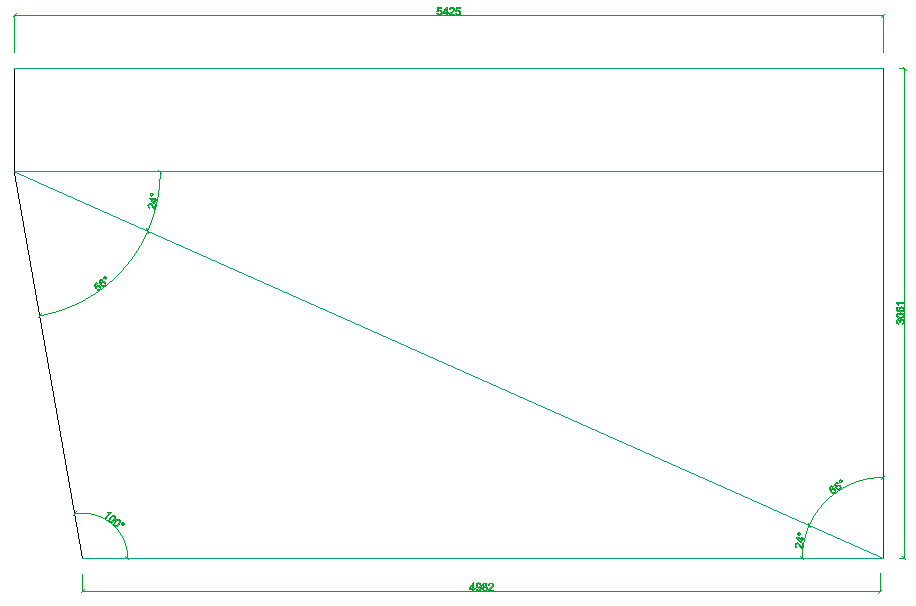
\includegraphics[width=0.8\textwidth]{image34}
	\caption{Vista laterale: Guscio di protezione}
	\label{fig:mesh1}
\end{figure}

\begin{figure}[H]
	\centering
	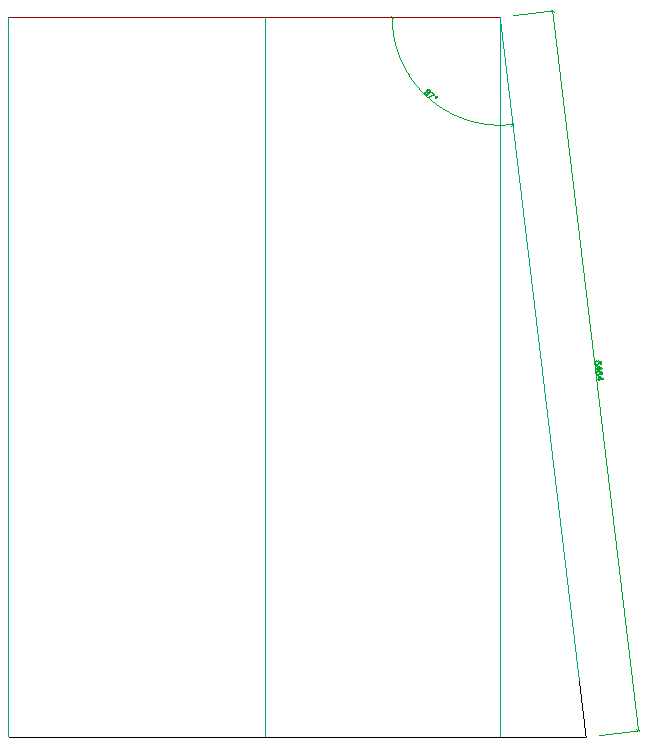
\includegraphics[width=0.5\textwidth]{image32}
	\caption{Prospetto posteriore}
	\label{fig:mesh1}
\end{figure}


\subsection{Analisi delle indicazione ergonomiche relative ai moduli costituenti il bancone da lavoro }

il bar si può suddividere in quattro sotto-aree funzionali: piano di servizio,piano di lavoro, sotto banco  e retrobanco.

Il piano di servizio è posizionato poco più in alto rispetto a quello di lavoro. Può essere rivestito nel materiale che si preferisce, in linea con lo stile del locale. 
È l’elemento di comunicazione tra cliente e barman ed è l’area dove vengono servite le preparazioni e disposti gli snack per gli aperitivi.
L’altezza totale del banco equivale all'altezza della bancalina, generalmente realizzata in marmo/pietra/corian o acciaio  = mm 1150 da terra. 

\begin{figure}[H]
	\centering
	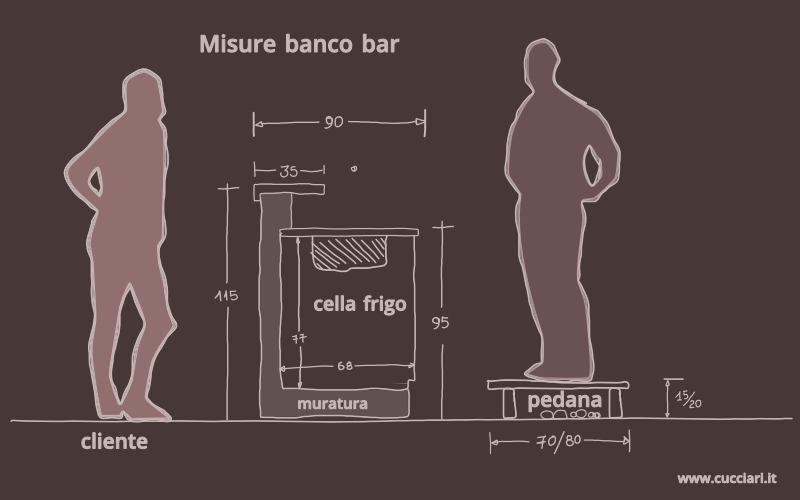
\includegraphics[width=0.8\textwidth]{image39}
	\caption{aaa}
	\label{fig:mesh1}
\end{figure}

Il piano di lavoro è la parte in cui vengono posizionate le attrezzature del bar utilizzate più spesso e meno ingombranti ed è appunto la zona in cui il barman prepara bevande e snack. L’altezza del piano di lavoro è di  mm 950 da terra, in genere realizzato in acciaio inox. 
È qui che generalmente trova posto anche il lavello con acqua corrente e uno spazio per bottiglie di uso frequente.

Nel sottobanco trovano posto tutte quelle attrezzature più ingombranti, utilizzate quotidianamente e adibite soprattutto alla conservazione delle bevande e al lavaggio: tra questi rientrano il frigorifero, la macchina per il ghiaccio, la lavabicchieri o la lavastoviglie professionale. L’apertura dei vani refrigerati avviene attraverso sportelli o cassetti, interamente  in acciaio inox.

Nel retrobanco del bar viene allestito il reparto caffetteria e espositore.
Il retrobanco può essere neutro o refrigerato e composto da un numero variabile di armadietti con sportelli o cassetti, si possono dividere più o meno in due parti.
Generalmente si distingue in due sezioni principali:
Retro espositivo


\begin{figure}[H]
	\captionsetup[subfloat]{farskip=2pt,captionskip=8pt}
	\centering
	\subfloat[Retro espositivo]{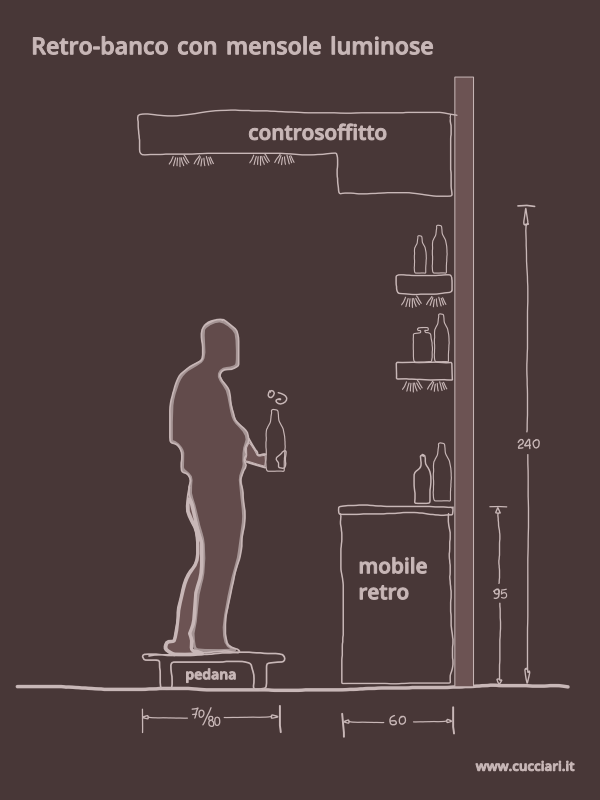
\includegraphics[width=6cm]{image46}}
	\hspace{1cm}
	\subfloat[Retro macchina caffè]{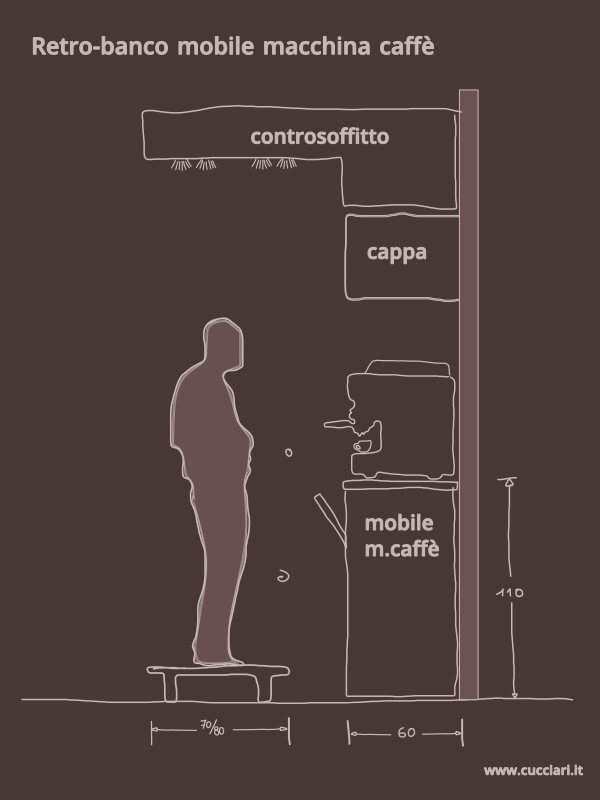
\includegraphics[width=6cm]{image8}}
	
	\caption{Retrobancone}
	\label{fig:imagesizes}
\end{figure}


Retro multiuso e bottiglie. Composto da mobile base e da un'alzata su cui si applicano le mensole portabottiglie o i fondali attrezzati per vari servizi 



troviamo: cassetti, macina-caffè,  tramoggia per i fondi del caffè, spazzatura, uno spazio per la lavastoviglie oppure il produttore di ghiaccio, un vano per l’addolcitore e la pompa macchina caffè.

